% --------------------------------------------------------------
% This is all preamble stuff that you don't have to worry about.
% Head down to where it says "Start here"
% --------------------------------------------------------------

\documentclass[12pt]{article}

\usepackage[margin=1in]{geometry} 
\usepackage{amsmath,amsthm,amssymb}
\usepackage{color}
%\usepackage{tikz, pgfplots}
\usepackage{graphicx}
\usepackage{epstopdf} %converting to PDF
\usepackage{subcaption}
\usepackage{listings}

\makeatletter

\renewcommand\section{\@startsection {section}{1}{\z@}%
	{-3.5ex \@plus -1ex \@minus -.2ex}%
	{2.3ex \@plus.2ex}%
	{\normalfont\large\bfseries}}% from \Large
\renewcommand\subsection{\@startsection{subsection}{2}{\z@}%
	{-3.25ex\@plus -1ex \@minus -.2ex}%
	{1.5ex \@plus .2ex}%
	{\normalfont\large\bfseries}}% from \large
\makeatother

\begin{document}
	
	% --------------------------------------------------------------
	%                         Start here
	% --------------------------------------------------------------
	
	%\renewcommand{\qedsymbol}{\filledbox}
	
	\title{\textbf{Statistical Learning Methods Exercise \#{2}}\\
	Universit{\'e} de Neuch\^{a}tel}%replace X with the appropriate number
	\author{{Lin Bai, 09935404}} %replace with your name
	
	\maketitle

	%%%%%%%%%%%%%%%%%%%%%%%%%%%%%%%%%%%%%%%%%%%%%%%%%%%%%%%%%%%%%%%%%%%%%%%%%%%%%%%%%%%
	%%%%%%   question 1
	%%%%%%%%%%%%%%%%%%%%%%%%%%%%%%%%%%%%%%%%%%%%%%%%%%%%%%%%%%%%%%%%%%%%%%%%%%%%%%%%%%%
	\section{Solution to question 1}
	\lstset{language=R}
	\lstset{frame=lines}
	\lstset{label={lst:code_direct}}
	\lstset{basicstyle=\footnotesize\ttfamily}
	\begin{lstlisting}[breaklines=true]
	carseatDataFrame <- read.table("Carseats.txt", 
	                               header=TRUE, sep="")
	
	carseatDataFrame$Color="black"
	carseatDataFrame$Color[carseatDataFrame$Price>180] = 'red'
	carseatDataFrame$Color[carseatDataFrame$Price<40] = 'red'
	carseatDataFrame$Color[carseatDataFrame$Sales>18] = 'red'
	
	plot(carseatDataFrame$Sales, carseatDataFrame$Price, 
	     main = "Car_seats_Sales-Price_Plot", 
	     xlab = "Sales", ylab = "Price", 
	     col = carseatDataFrame$Color)
	\end{lstlisting}
	
	\begin{figure}[htbp]
		\centering
		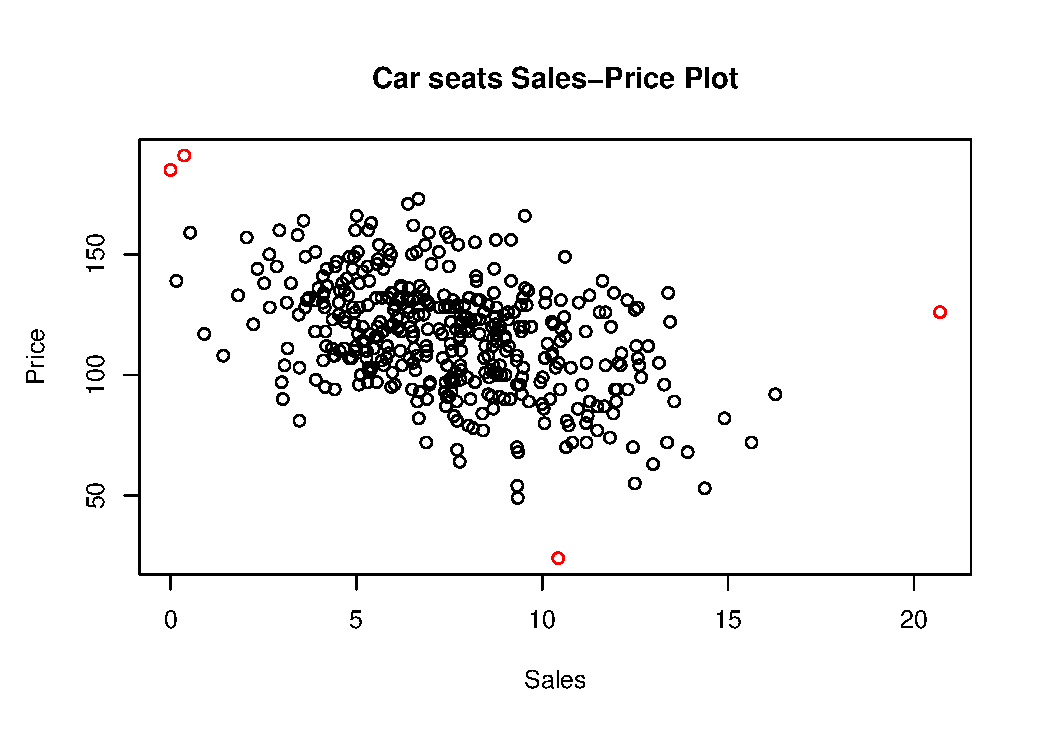
\includegraphics[width=0.7\textwidth]{figure1.eps}
		\caption{car seat sales-price plot}
	\end{figure}
\newpage
	%%%%%%%%%%%%%%%%%%%%%%%%%%%%%%%%%%%%%%%%%%%%%%%%%%%%%%%%%%%%%%%%%%%%%%%%%%%%%%%%%%%
	%%%%%%   question 2
	%%%%%%%%%%%%%%%%%%%%%%%%%%%%%%%%%%%%%%%%%%%%%%%%%%%%%%%%%%%%%%%%%%%%%%%%%%%%%%%%%%%
	\section{Solution to question 2}
	\lstset{language=R}
	\lstset{frame=lines}
	\lstset{label={lst:code_direct}}
	\lstset{basicstyle=\footnotesize\ttfamily}
	\begin{lstlisting}[breaklines=true]
	educationDataFrame <- read.table("Education.txt", 
	                                 header=TRUE, 
	                                 sep="")
	subUS <- subset(educationDataFrame, Country=="US")
	subCA <- subset(educationDataFrame, Country=="Canada")
	
	xUS <- subUS$Education
	yUS <- subUS$Wage
	colUS <- 'red'
	
	xCA <- subCA$Education
	yCA <- subCA$Wage
	colCA <- 'blue'
	
	plot(xUS, yUS, col= colUS, xlab = "Education", ylab = "Wage")
	points(xCA, yCA, col= colCA)
	
	legend(8, 8000, 
	       c("US", "Canada"), 
	       lwd=c(2.5,2.5), 
	       col=c("red","blue"))
	\end{lstlisting}
	
	\begin{figure}[htbp]
		\centering
		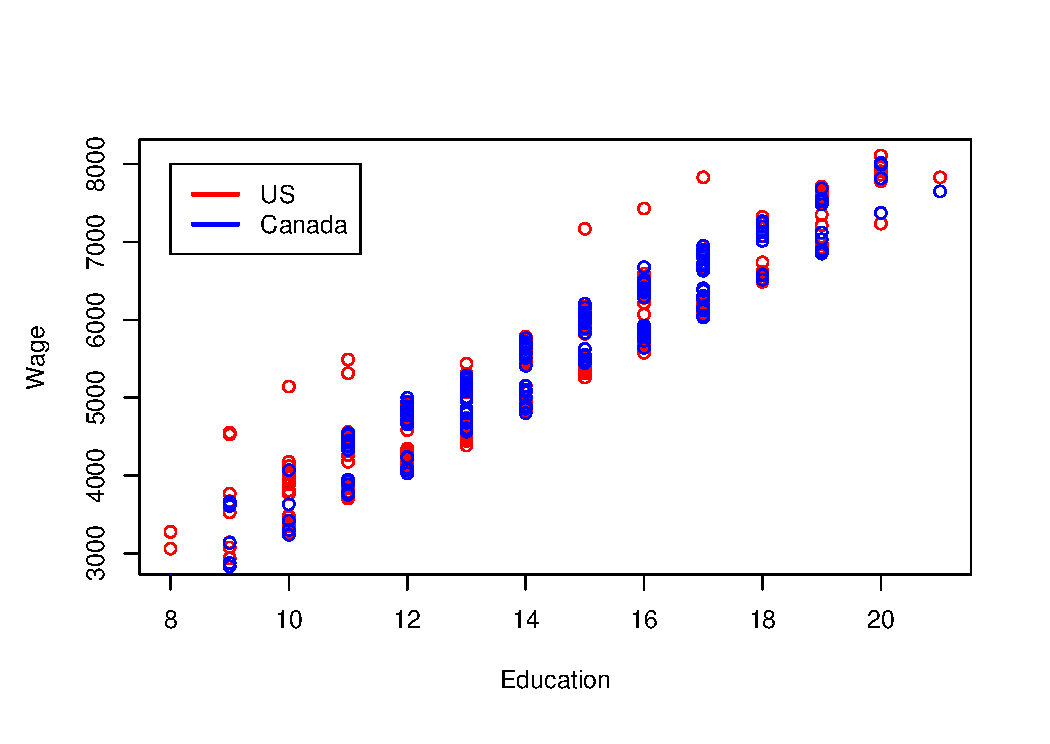
\includegraphics[width=0.7\textwidth]{figure2.eps}
		\caption{education wage plot}
	\end{figure}
\newpage
	%%%%%%%%%%%%%%%%%%%%%%%%%%%%%%%%%%%%%%%%%%%%%%%%%%%%%%%%%%%%%%%%%%%%%%%%%%%%%%%%%%%
	%%%%%%   question 3
	%%%%%%%%%%%%%%%%%%%%%%%%%%%%%%%%%%%%%%%%%%%%%%%%%%%%%%%%%%%%%%%%%%%%%%%%%%%%%%%%%%%
	\section{Solution to question 3}
	The data need preprocessing. Time should be non-negative.\\
	\lstset{language=R}
	\lstset{frame=lines}
	\lstset{label={lst:code_direct}}
	\lstset{basicstyle=\footnotesize\ttfamily}
	\begin{lstlisting}[breaklines=true]
	mean20DataFrame <- read.table("Mean20.txt", 
	                              header = TRUE, sep = "")
	processed = subset(mean20DataFrame, !is.na(time) & time > 0) 
	summary(processed$time)
	\end{lstlisting}
	\noindent
	The mean is 7.008, median is 7.010, standard deviation is 0.07515598, the minimum is 6.850 and maximum is 7.120.\\

	%%%%%%%%%%%%%%%%%%%%%%%%%%%%%%%%%%%%%%%%%%%%%%%%%%%%%%%%%%%%%%%%%%%%%%%%%%%%%%%%%%%
	%%%%%%   question 4
	%%%%%%%%%%%%%%%%%%%%%%%%%%%%%%%%%%%%%%%%%%%%%%%%%%%%%%%%%%%%%%%%%%%%%%%%%%%%%%%%%%%
	\section{Solution to question 4}
	\lstset{language=R}
	\lstset{frame=lines}
	\lstset{label={lst:code_direct}}
	\lstset{basicstyle=\footnotesize\ttfamily}
	\begin{lstlisting}[breaklines=true]
	t.test(processed$time, mu = 7.05, alternative = "two.sided")
	
		One Sample t-test
	
	data:  processed$time
	t = -2.4992, df = 19, p-value = 0.02178
	alternative hypothesis: true mean is not equal to 7.05
	95 percent confidence interval:
	6.972826 7.043174
	sample estimates:
	mean of x 
	7.008 
	
	t.test(mean20DataFrame$time, mu = 7.05, alternative = "two.sided")
	
		One Sample t-test
	
	data:  mean20DataFrame$time
	t = -1.0626, df = 20, p-value = 0.3006
	alternative hypothesis: true mean is not equal to 7.05
	95 percent confidence interval:
	4.947647 7.733306
	sample estimates:
	mean of x 
	6.340476 
	
	\end{lstlisting}
	\noindent
	\textbf{Data without preprocess}: p-value is the possibility observing the test result under the null hypothesis, here p-value = 0.02178 $<$ 0.05.\\
	\textbf{Data with preprocess}: while, if using original values, the hypothesis is correct but the possibility is not high.

	%%%%%%%%%%%%%%%%%%%%%%%%%%%%%%%%%%%%%%%%%%%%%%%%%%%%%%%%%%%%%%%%%%%%%%%%%%%%%%%%%%%
	%%%%%%   question 5
	%%%%%%%%%%%%%%%%%%%%%%%%%%%%%%%%%%%%%%%%%%%%%%%%%%%%%%%%%%%%%%%%%%%%%%%%%%%%%%%%%%%
	\section{Solution to question 5}
	\lstset{language=R}
	\lstset{frame=lines}
	\lstset{label={lst:code_direct}}
	\lstset{basicstyle=\footnotesize\ttfamily}
	\begin{lstlisting}[breaklines=true]
	t.test(processed$time, mu = 7.05, alternative = "greater")
	
		One Sample t-test
	
	data:  processed$time
	t = -2.4992, df = 19, p-value = 0.9891
	alternative hypothesis: true mean is greater than 7.05
	95 percent confidence interval:
	6.978941      Inf
	sample estimates:
	mean of x 
	7.008 
	\end{lstlisting}
	The null hypothesis cannot be rejected, which means true mean is less then 7.05, therefore, John is wrong.	
	% --------------------------------------------------------------
	%     You don't have to mess with anything below this line.
	% --------------------------------------------------------------
	
\end{document}